% !TeX spellcheck = ca
% TIPUS DE DOCUMENT
\documentclass[a4paper,10pt]{article} 
% Permet canviar la mida del paper, la mida de la lletra...

% GEOMETRIA
%\usepackage[a4paper,bindingoffset=0.2in,%
%left=3cm,right=3cm,top=2.5cm,bottom=2.5cm,%
%footskip=.25in]{geometry} % Marges normals

\usepackage[a4paper,bindingoffset=0.2in,%
left=1in,right=1in,top=1in,bottom=1in,%
footskip=.25in]{geometry} % Marges estrets

% IDIOMA 
%\usepackage[catalan]{babel} %Fa que l'idioma del document sigui en català (p.ex. escriurà "Resum" enlloc de "Abstract")
\usepackage[english]{babel} %Fa que l'idioma del document sigui l'anglès

% ENCODING
\usepackage{cmap,lmodern}  % Útil tenir-ho sempre.
\usepackage[T1]{fontenc} % Millora els caràcters del pdf que es produeix
\usepackage[utf8]{inputenc} % Evita problemes amb què LaTeX no sàpiga llegir certs caràcters.
\usepackage{hyperref} % Permet que els links siguin clicables en lectors pdf

% IMATGES
% \usepackage{wrapfig,graphicx} % Permet afegir imatges
%\graphicspath{{Imatges/} % Si volem guardar totes les imatges en una carpeta (+ còmode)
\usepackage[font=small]{caption} % Peus de foto
% \usepackage{subcaption} % Subpeus de foto
% \usepackage{tikz}
% \usepackage{float}
% \usepackage{pgfplots}
% \usepackage{multirow}
\usepackage[labelfont=bf]{caption}
\usepackage{fancyhdr}
\usepackage{bm}
\usepackage{hyperref}
\usepackage{graphicx}
% \usepackage{gensymb}
\usepackage{amsmath}
\usepackage{amssymb}
% \usepackage{siunitx}
\usepackage{parskip}
% \usepackage{blindtext}
\usepackage{graphicx}
\usepackage[utf8]{inputenc}
% \usepackage{multirow}
\usepackage{longtable}
\usepackage{fancyvrb}
\usepackage{xcolor}
\usepackage{subcaption}
\usepackage{wrapfig}
\usepackage{fancyhdr}
\usepackage{listings}
\usepackage{color}
\usepackage{siunitx}
	
% EQUACIONS
% \usepackage{mathtools,amsmath,amssymb,systeme,braket} % Diverses eines d'equacions
	
% OTROS
\setlength{\parindent}{0em}   % Controla la indentació de la primera línia de cada paràgraf
%\setlength{\parskip}{0.3em}   % Controla la mida de 'espaiat entre paràgrafs
%\usepackage{enumitem} %Permet el control sobre llistes
%\setlist{noitemsep,nolistsep} % Controla l'espaiat entre elements de llista (requereix el paquet enumitem)
	
\definecolor{dkgreen}{rgb}{0,0.6,0}
\definecolor{gray}{rgb}{0.5,0.5,0.5}
\definecolor{mauve}{rgb}{0.58,0,0.82}

\lstset{frame=tb,
	language=Fortran,
	aboveskip=3mm,
	belowskip=3mm,
	showstringspaces=false,
	columns=flexible,
	basicstyle={\small\ttfamily},
	numbers=none,
	numberstyle=\tiny\color{gray},
	keywordstyle=\color{blue},
	commentstyle=\color{dkgreen},
	stringstyle=\color{mauve},
	breaklines=true,
	breakatwhitespace=true
	tabsize=3
}	
	
\usepackage{fancyhdr}
\usepackage{tcolorbox}% TIPUS DE DOCUMENT
	
\pagestyle{fancy}
\fancyhf{}
\rhead{Aina Gaya}
\lhead{Pràctiques de models QM i MM}
\cfoot{\thepage}
	%
	%opening
\title{\textsc{{\large Molecular modelling } \\ Analysis of properties of a Lennard-Jones liquid } \\  {\small Molecular Dynamics}}
\author{Aina Gaya Àvila \\ {\small Lecturer: Carles Calero }}
	
\begin{document}
		
\maketitle

\begin{abstract}
	S'efectuen simulacions de dinàmica molecular en un sistema de 125 partícules interactuant a través d'un potencial de Lennard-Jones. S'apliquen condicions periòdiques de contorn per simular un sistema infinit. En primer lloc, s'efectuen simulacions en un sistema aïllat emprant els integradors de Verlet i d'Euler. La densitat del sistema es fixa a $\rho' = 0.7$ La temperatura d'equilibri reduïda obtinguda és $T' = 85.33$. Es pot veure con Euler és més inestable. A continuació s'efectuen simulacions fixant la temperatura amb un termòstat Andersen. Es varia la densitat i s'observa una transició de fase. 
\end{abstract}

\section{Introducció: Simulacions de dinàmica molecular}
El model microscòpic més senzill per simular una substància capaç d'existir tant en estat sòlid, líquid com gasós està basat en partícules esfèriques que interactuen entre elles. Aquesta interacció es modelitza tenint en compte dues característiques:
\begin{itemize}
	\item La resistència a la compressió, és a dir, que cada partícula ocupa el seu espai i a curt abast la interacció és repulsiva. És el principi d'exclusió de Pauli.
	\item Les forces de Van der Waals entre àtoms als estats sòlid i líquid, que tendeixen a apropar les partícules.
\end{itemize}

El potencial més emprat per simular el descrit anteriorment és el de Lennard-Jones. Per descriure el potencial entre dues particules $i$ i $j$, localitzades a $r_i$ i $r_j$, pren la forma següent:

$$ u(r_{ij}) = 4 \epsilon \left[ \left( \frac{\sigma}{r_{ij}}\right)^{12} - \left( \frac{\sigma}{r_{ij}}\right)^{6} \right] $$

On 

\begin{itemize}
	\item $r_{ij} = | r_i - r_j | $ és la distància entre partícules.
	\item $\sigma$ defineix la mida de la partícula.
	\item $\epsilon$ és la profunditat del potencial. És una mesura de la magnitud de la interacció.
\end{itemize}

L'objectiu d'aquest projecte és dur a terme una simulació d'un líquid de Lennard-Jones per estudiar-ne les seves propietats. A cada pas de temps es calcularà la magnitud i la direcció de la interacció entre les partícules i es farà evolucionar el sistema en funció d'aquestes. L'hamiltonià del sistema serà:

\begin{equation}
	\mathcal{H} = \sum_{i}^{N} \frac{p_i}{2 m_i} + U(r_1, r_2, ..., r_N)
\end{equation}

El primer terme correspon a l'energia cinètica, i el segon a l'energia potencial. En el segon terme es tenen en compte tant els efectes d'un camp extern (inexistent en el nostre cas) com l'efecte de les interaccions entre les partícules. En aquesta pràctica només es tindran en compte les interaccions entre parelles de partícules, i aquestes vindran descrites pel potencial de Lennard-Jones. Les interaccions entre tres, quatre, o més partícules són més costoses de calcular i la seva contribució és menys rellevant. 

\begin{figure}
	\centering
	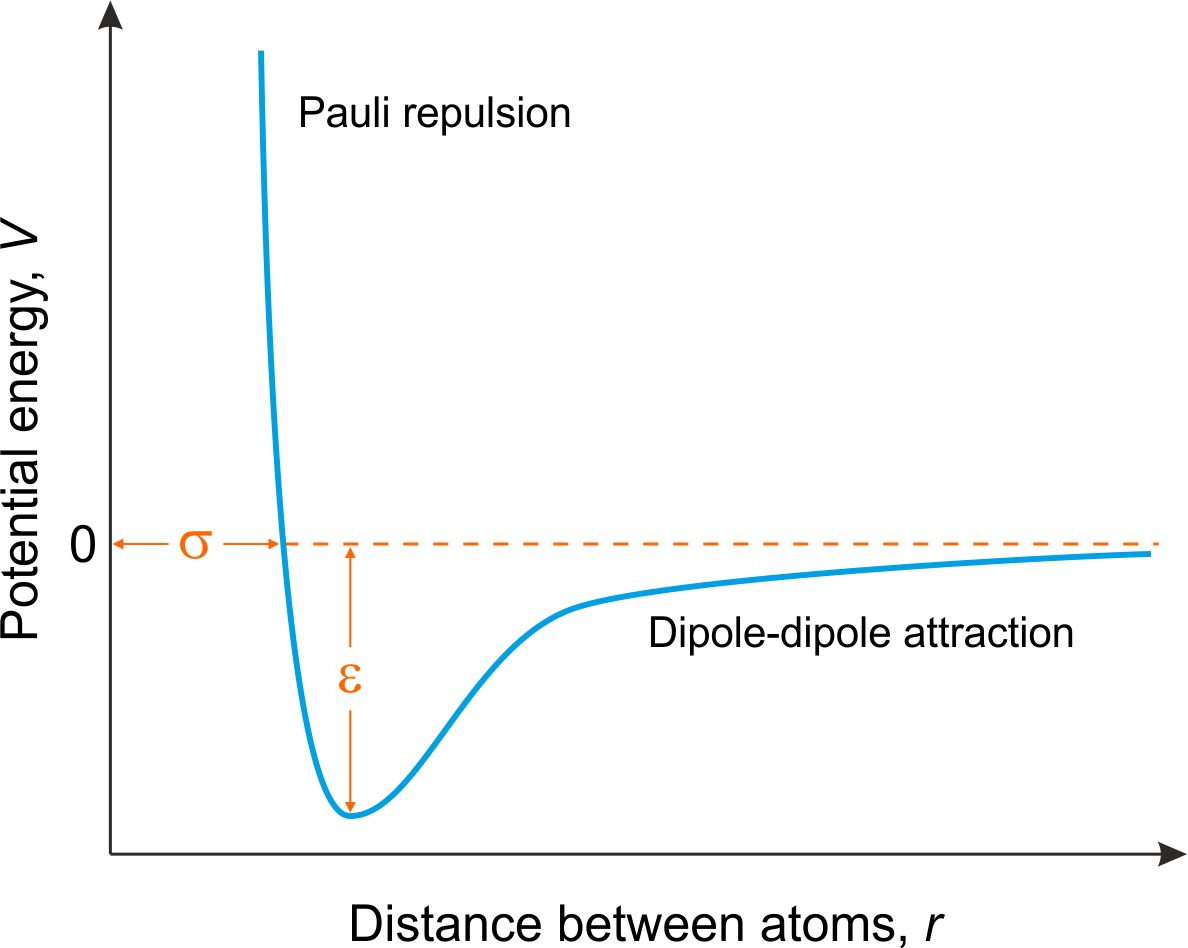
\includegraphics[width=0.7\linewidth]{lennard-jones_potential}
	\caption{Potencial de Lennard-Jones.}
	\label{fig:lennard-jonespotential}
\end{figure}


%(a) Describe in detail the different parts of the code. 


% How do you initialize the system of particles (and set the density)? 
Estudiarem un sistema de $N=125$ partícules. L'altre paràmetres que definirà el sistema serà la densitat. Totes les simulacions estan dutes a terme amb Fortran90, i la part de processament de dades s'ha fet combinant Python, Gnuplot i Bash

El sistema és inicialitzat emprant una estructura cúbica simple (SC), i per tant, en podem calcular el volum $V$ i la llargada de cada un dels costats $L$ i la distància entre partícules $a$:

$$ V = \frac{N}{\rho} \qquad L = V^{1/3} \qquad a = \frac{L}{N^{1/3}} $$

Sabent la distància entre partícules, inicialitzem el sistema amb la subrutina que es troba a \ref{annex:inicialitzacio}, que situa les partícules de manera que formin una estructura SC.

% What integrator do you use?
\subsection{Integradors}
L'integrador que emprarem per solucionar les equacions de Newton que regeixen aquest sistemà serà, principalment, el \textit{velocity Verlet}. La implementació d'aquest algoritme és la següent:

\begin{itemize}
	\item Es disposa de les posicions i les velocitats de les partícules, que han estat calculades al pas anterior (o s'empren les condicions inicials si és el primer pas de temps).
	\item Es calcula la força $f$ sobre cada partícula.
	\item Es calcula la posició emprant la velocitat: $r (t + \Delta t) = r(t) + v(t) \Delta t + \frac{f(t)}{2m}\Delta t ^2$.
	\item Es calcula  la força sobre cada partícula a $t + \Delta t$ emprant la nova distribució de partícules. 
	
	\item Es calcula la velocitat a $t + \Delta t$: $v(t+\Delta t) = v(t) + \frac{f(t) + f(t + \Delta t)}{2m} \Delta t$.

\end{itemize}

El compararem també amb el mètode d'Euler, que a cada pas de temps calcula les posicions i les velocitats de manera explícita:
\begin{equation}
	r_i (t+\Delta t) = r_i(t) + v_i(t) \Delta t + \frac{f_i(t)}{2m_i}\Delta t^2 \qquad v_i (t + \Delta t) = v_i (t) + \frac{f_i(t)}{m_i} \Delta t
\end{equation}

\subsection{Condicions periòdiques de contorn}
%  How do you implement periodic boundary conditions? 
Per simular que estem tractant un sistema major (infinit) cal implementar condicions periòdiques de contorn. Això genera infinites còpies de les nostres partícules i elimina l'efecte de les parets. La implementació es troba a \ref{annex:pbc}. És important mencionar que les condicions periòdiques de contorn condicionen el pas temporal ($\Delta t$) que podem emprar. Posem per exemple dues partícules molt properes que s'estan repel·lint. El desplaçament provocat per la força repulsiva que exerceix cada una sobre l'altre és proporcional a $f_i \delta t^2$. Cal evitar que aquest desplaçament sigui massa gran ja que si  sobrepassa $L/4$, degut a les condicions periòdiques de contorn, en el següent pas de temps es trobarien més a prop del que estaven, i això comporta inestabilitats.

% How do you control the temperature (how do you implement the thermostat)? 
\subsection{Control de la temperatura}
Inicialitzarem el sistema partint d'una estructura cúbica simple en la qual la velocitat de cada partícula seguirà una distribució bimodal (amb dos pics) que correspongui a una temperatura reduïda $T' = 100 $. Com que la temperatura instantània $T_{inst}$, del principi d'equipartició, és:

\begin{equation}
	T_{inst} = \frac{2}{N_f k_b} K_e
\end{equation}

Tenint en compte que l'energia cinètica és $K_e = \frac{1}{2} m v^2$, podem veure que la velocitat de les partícules a una temperatura instantània fixa és:

$$ v^2 = \frac{T N_f k_b}{m} \to v_i = \pm \sqrt{\frac{T k_b}{m}}  $$

Aleshores, per inicialitzar el sistema, assignarem aleatòriament $v_{+}$ o $v_{-}$ a cada component de cada partícula.

Per simular un sistema que pertanyi a la col·lectivitat canònica (nombre de partícules, volum i temperatura determinats) s'empra un termòstat Andersen. Aquest termòstat s'empra molt en dinàmica molecular. Consisteix en reassignar, amb una certa probabilitat, la velocitat d'una partícula seguint una distribució gaussiana, centrada la temperatura a la qual es vol mantenir el sistema. Per generar aquests nombres aleatoris s'empra un generador Box-Müller.

% What units do you use for the Lennard-Jones interactions? 
\subsection{Unitats reduïdes}
Per evitar treballar amb nombres molt grans o molt petits, que podrien estar fora del rang depenent de la precisió amb la que es treballi, es defineixen les unitats reduïdes. A més, això simplifica substancialment les equacions, ja que els paràmetres que defineixen el model són absorbides per les unitats. Emperò, el motiu principal per definir les unitats reduïdes és que un sol model és capaç de descriure múltiples problemes, ja que les propietats que es dedueixen emprant les unitats arbitràries es poden escalar a les unitats físiques apropiades per cada un dels problemes. Per problemes de Lennard-Jones s'escullen respectivament $\sigma$, $m$ i $\varepsilon$ com a unitats de longitud, massa i energia.

La distància reduïda serà aleshores $r' = r/\sigma$, l'energia $u' = u/\varepsilon$, la massa $m' = 1$. D'aquestes se'n pot derivar el temps:

$$ [F] = [m][a] \to \frac{[E]}{[r]} = [m]\frac{[r]}{[t]^2} \to [t] = \frac{1}{[r]}\sqrt{\frac{[E]}{[m]}} \to t' =  \frac{t}{\sigma}\sqrt{\frac{\epsilon}{m}} $$ 

La temperatura:

$$ k_B = \frac{[E]}{[T]} \to T' = T \frac{k_B}{\epsilon} $$

La densitat:

\begin{equation}
	[\rho] = \frac{[m]}{[V]} \to \rho' = \rho \frac{\sigma^3}{m}
\end{equation} 

I la pressió:

\begin{equation}
	[P] = \frac{[F]}{[r]^2} = \frac{[E]/[r]}{[r]^2} = \frac{\varepsilon}{\sigma^3} \to P' = P \frac{\sigma^3}{\varepsilon}
\end{equation}



% What cut-off do you use for the interactions (and why)? 
\subsection{Optimizacions: \textit{cutoff} i truncació}
Com que estem treballant amb condicions periòdiques de contorn cada partícula pot interactuar amb infinites partícules, ja que hi ha infinites imatges de cada partícula. Per evitar aquesta suma infinita i a més optimitzar els càlculs computacionals, només es calculen les forces entre les partícules que estan a menor distància que una distància que anomenarem \textit{cutoff} ($r_c$). Definirem $r_c' = 2.5$ ja que com es pot veure a la figura \ref{fig:lennard-jonespotential}, a distàncies majors la contribució és gairebé nul·la. El potencial doncs seria:

$$ u^{cut}(r) = \left\{ \begin{array}{lcc} u^{LJ}(r), & \text{if } r \leq r_c \\ 0,  & \text{if } < r_c  \end{array} \right.$$

Aquesta truncació dóna lloc a un salt discontinuu, que dóna problemes en calcular les forces derivades d'aquest potencial. És per aquest motiu que el potencial escollit per la nostra simulació fa servir tant un \textit{cutoff} com un \textit{shift}, que porta a un potencial continuu: 

\begin{equation}
	u^{cut}(r) = \left\{ \begin{array}{lcc} u^{LJ}(r) - u^{LJ}(r_c), & \text{if } r \leq r_c \\ 0,  & \text{if } < r_c  \end{array} \right.
\end{equation}	

\section{Simulació d'un sistema aïllat}
Per comprovar que la física del sistema del sistema que estem descrivint és consistent, en primer lloc durem a terme una simulació d'un sistema aïllat, que no està en contacte amb un bany tèrmic. Situarem 125 partícules en una estructura cúbica simple (5x5x5) amb una distribució de velocitats bimodal compatible amb una temperatura instantania $T'=100$. Emprem  $\rho = 0.7 m\sigma^3$. Hem estudiat el comportament del sistema al llarg de $t' = 1$ fent servir diferents passos de temps: $\Delta t = 10^{-3}$, $\Delta t = 10^{-4}$ i $\Delta t = 10^{-5}$. Per intervals majors s'han trobat inestabilitats i vist que la conservació de l'energia es compleix en aquesta escala, no s'han considerat intervals menors, ja que són més costosos computacionalment. 

\subsection{Conservació de l'energia}

Els resultats obtinguts per diferents passos de temps per l'integrador de velocity Verlet es mostra a la figura \ref{fig:energyverlet}. En tots ells s'observa que l'energia del sistema es conserva. També es veu com el sistema s'equilibra en els primers instants, ja que l'energia potencial augmenta i la cinètica disminueix. Això succeeix perquè les partícules, que inicialment tenien la velocitat corresponent a $T'=100$, son parcialment frenades per la interacció de Lennard-Jones. Un cop s'equilibra el sistema, hi ha oscil·lacions a l'energia potencial i a la cinètica però l'energia total es manté constant. 

\begin{figure}
	\centering
	\begin{subfigure}{0.45\linewidth}
		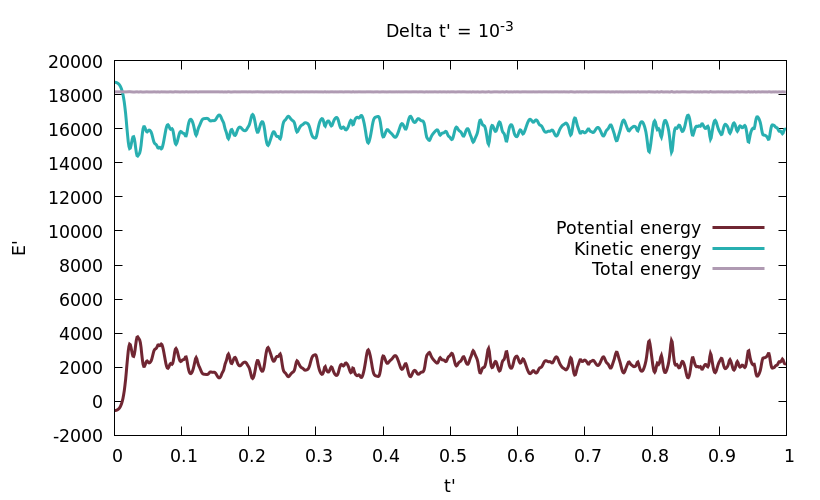
\includegraphics[width=\linewidth]{energy_verlet_1}
		\caption{$\Delta t = 10^{-3}$}
		\label{fig:energyverlet1}
	\end{subfigure}
	\begin{subfigure}{0.45\linewidth}
		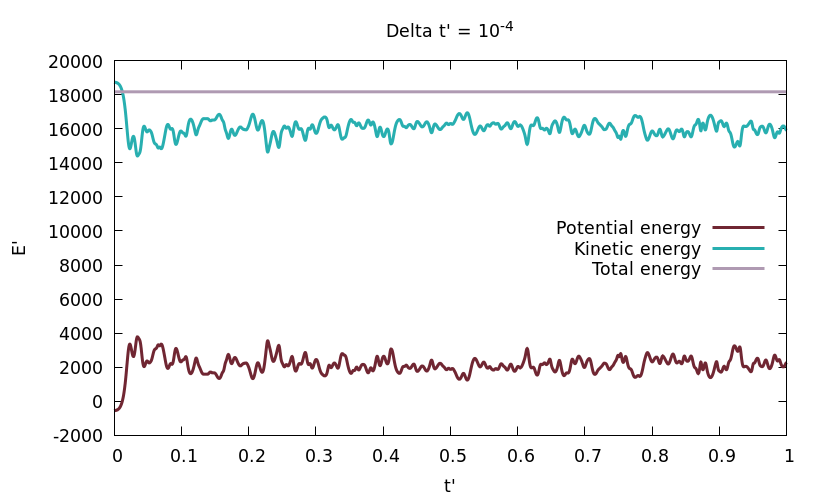
\includegraphics[width=\linewidth]{energy_verlet_2}
		\caption{$\Delta t = 10^{-4}$}
		\label{fig:energyverlet2}
	\end{subfigure}
	\begin{subfigure}{0.45\linewidth}
		% CHANGE THIS!!!
		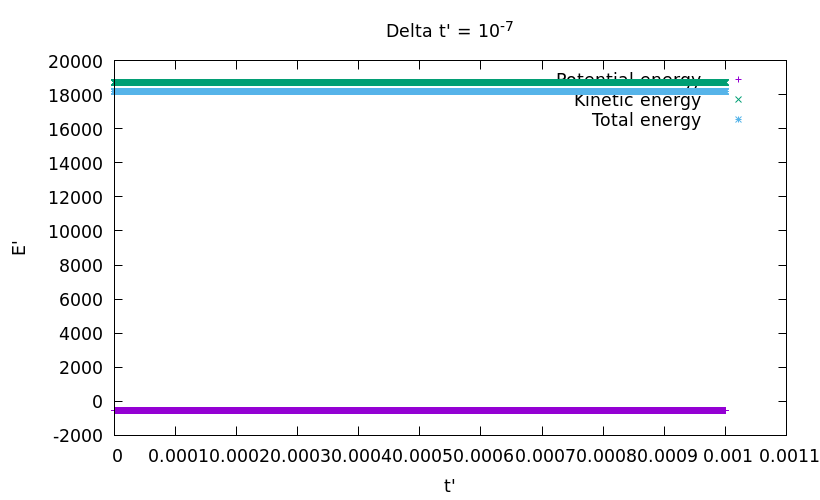
\includegraphics[width=\linewidth]{energy_verlet_3} 
		\caption{$\Delta t = 10^{-5}$}
		\label{fig:energyverlet3}
	\end{subfigure}
	\caption{Energia potencial, cinètica i total en una simulació on s'empra l'integrador velocity Verlet, per diversos passos de temps.}
	\label{fig:energyverlet}
\end{figure}

Per l'integrador Euler s'han fet servir els mateixos passos de temps, però s'ha integrat en un interval menor, que per \textit{velocity Verlet} ha estat suficnet per equilibrar el sistema. Els resultats es poden veure a \ref{fig:energyeuler}. Pel pas de temps més gran a \ref{fig:energyeuler1} podem veure com l'energia del sistema no es conserva i va augmentant. Amb el pas un ordre de magnitud menor la situació millora, però l'energia total segueix augmentant. Pel darrer pas de temps que hem estudiat el sistema sembla més estable i l'energia es conserva.

\begin{figure}
	\centering
	\begin{subfigure}{0.45\linewidth}
		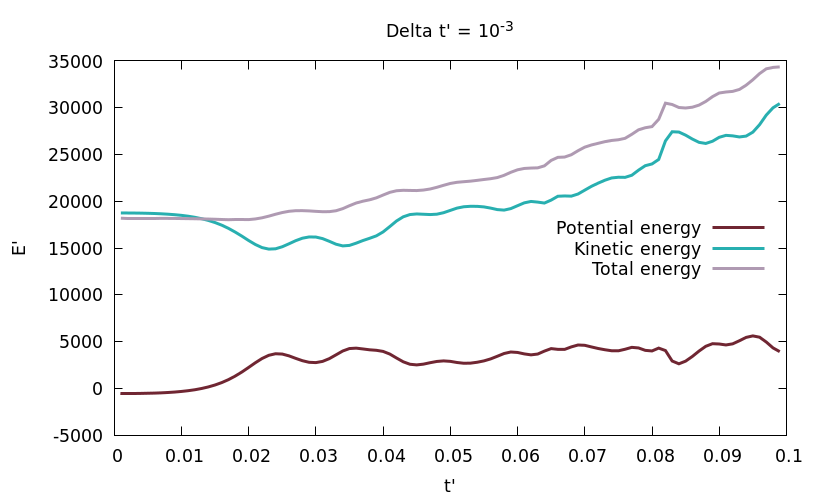
\includegraphics[width=\linewidth]{energy_euler_1}
		\caption{$\Delta t = 10^{-3}$}
		\label{fig:energyeuler1}
	\end{subfigure}
	\begin{subfigure}{0.45\linewidth}
		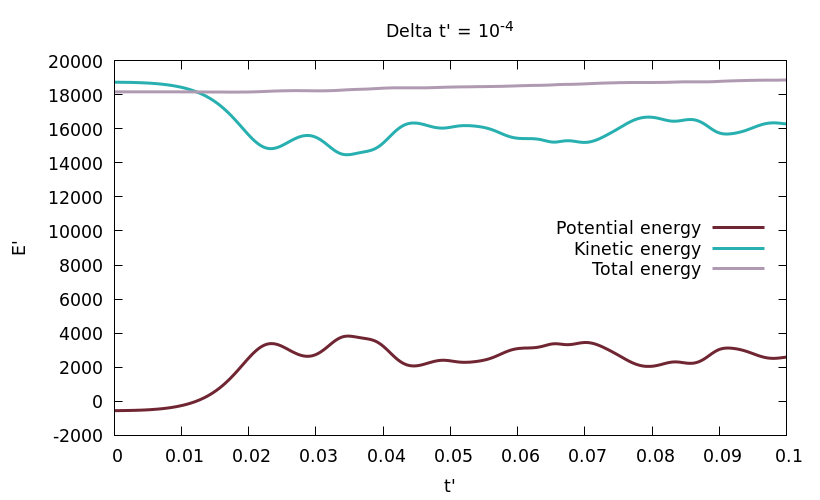
\includegraphics[width=\linewidth]{energy_euler_2}
		\caption{$\Delta t = 10^{-4}$}
		\label{fig:energyeuler2}
	\end{subfigure}
	\begin{subfigure}{0.45\linewidth}
		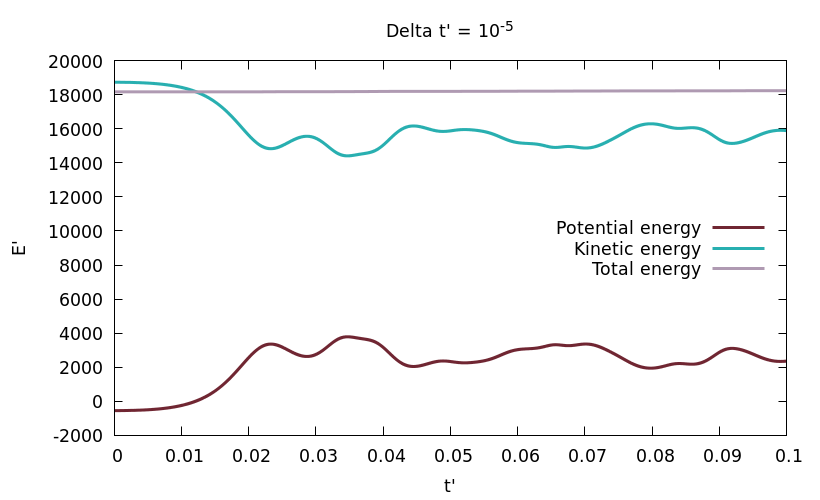
\includegraphics[width=\linewidth]{energy_euler_3} 
		\caption{$\Delta t = 10^{-5}$}
		\label{fig:energyeuler3}
	\end{subfigure}
	\caption{Energia potencial, cinètica i total en una simulació on s'empra l'integrador d'Euler, per diversos passos de temps.}
	\label{fig:energyeuler}
\end{figure}

\subsection{Conservació del moment}

A les figures \ref{fig:momentumverlet} i \ref{fig:momentumeuler} podem veure l'evolució del moment durant la simulació. Les oscil·lacions per ambdós integradors són a ordres molt petits i per tant són menyspreables. Podem afirmar que en les simulacions dutes a terme el moment es conserva.

\begin{figure}[h]
	\centering
	\begin{subfigure}{0.3\linewidth}
		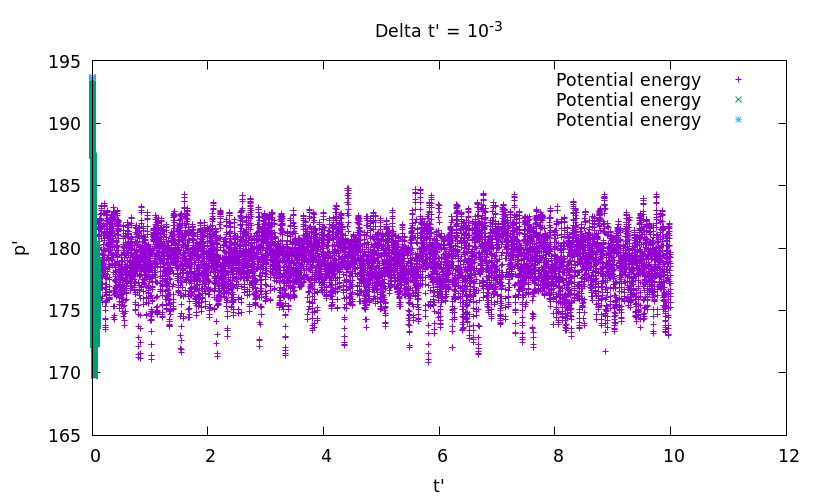
\includegraphics[width=\linewidth]{momentum_verlet_1}
		\caption{$\Delta t = 10^{-3}$}
		\label{fig:momentumverlet1}
	\end{subfigure}
	\begin{subfigure}{0.3\linewidth}
		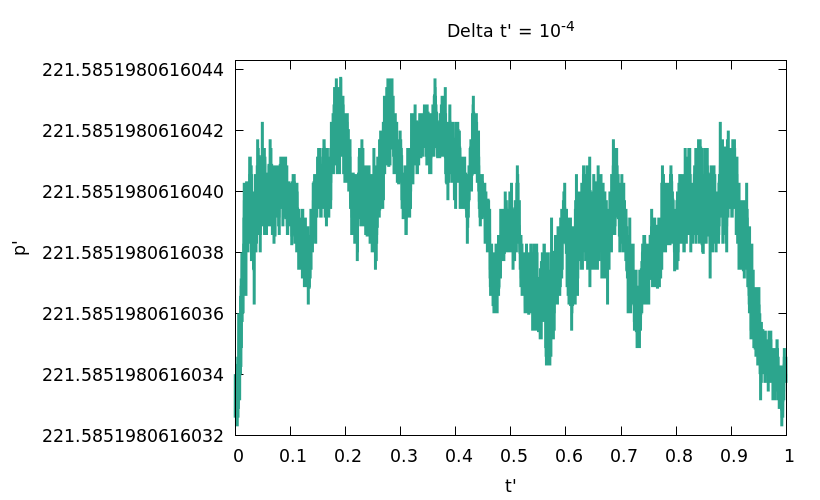
\includegraphics[width=\linewidth]{momentum_verlet_2}
		\caption{$\Delta t = 10^{-4}$}
		\label{fig:momentumverlet2}
	\end{subfigure}
	\begin{subfigure}{0.3\linewidth}
		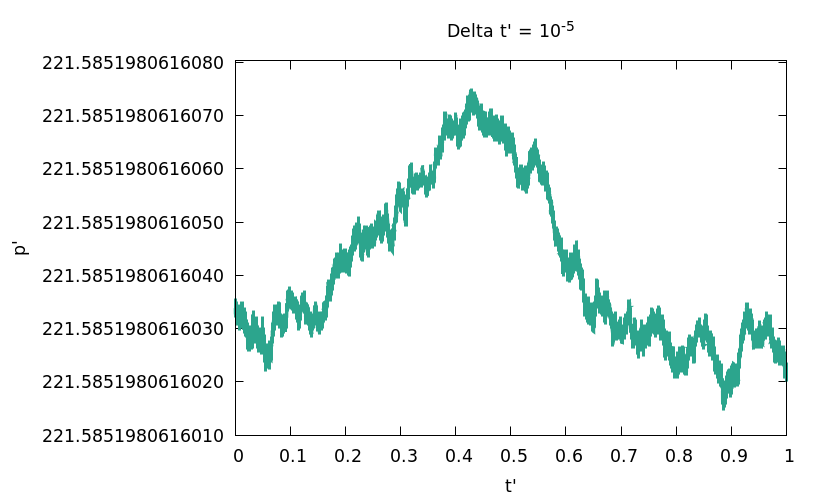
\includegraphics[width=\linewidth]{momentum_verlet_3} 
		\caption{$\Delta t = 10^{-5}$}
		\label{fig:momentumverlet3}
	\end{subfigure}
	\caption{Moment total en simulació on s'empra l'integrador velocity Verlet, per diversos passos de temps. El moment es considera constant, ja que s'ha d'anar a escales molt petites per veure'n les oscil·lacions.}
	\label{fig:momentumverlet}
\end{figure}

\begin{figure}[h]
	\centering
	\begin{subfigure}{0.3\linewidth}
		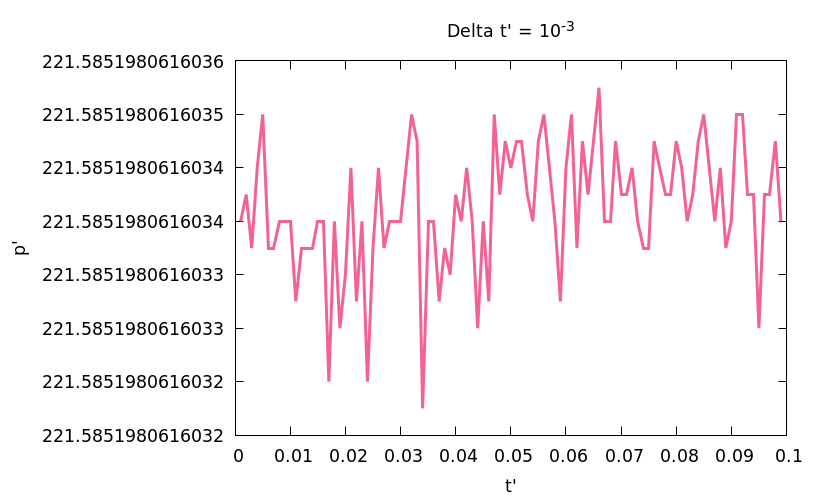
\includegraphics[width=\linewidth]{momentum_euler_1}
		\caption{$\Delta t = 10^{-3}$}
		\label{fig:momentumeuler1}
	\end{subfigure}
	\begin{subfigure}{0.3\linewidth}
		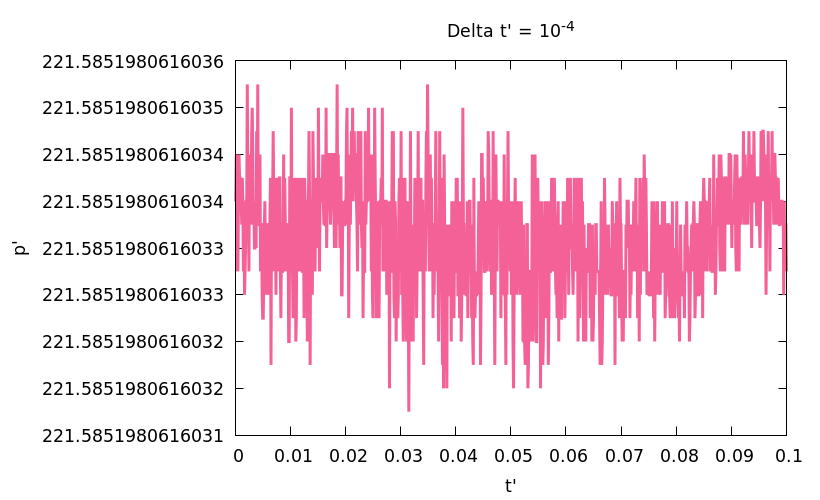
\includegraphics[width=\linewidth]{momentum_euler_2}
		\caption{$\Delta t = 10^{-4}$}
		\label{fig:momentumeuler2}
	\end{subfigure}
	\begin{subfigure}{0.3\linewidth}
		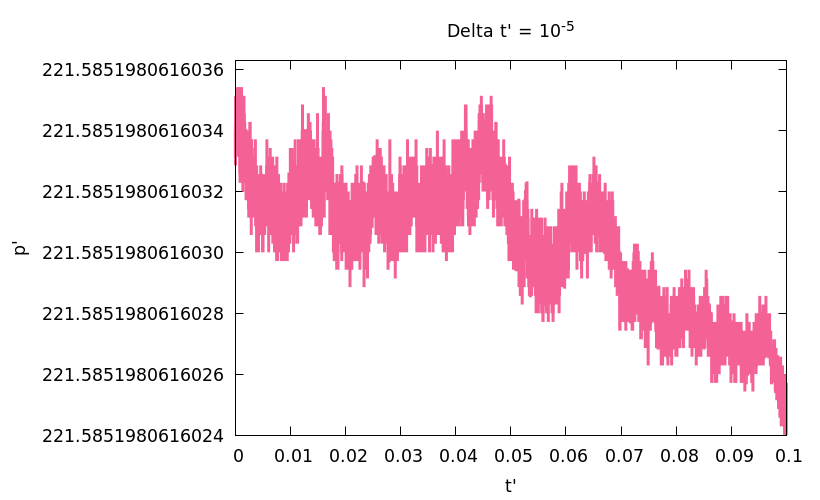
\includegraphics[width=\linewidth]{momentum_euler_3} 
		\caption{$\Delta t = 10^{-5}$}
		\label{fig:momentumeuler3}
	\end{subfigure}
	\caption{Moment total en simulació on s'empra l'integrador Euler, per diversos passos de temps. El moment es considera constant, ja que s'ha d'anar a escales molt petites per veure'n les oscil·lacions.}
	\label{fig:momentumeuler}
\end{figure}

\subsection{Distribució de velocitats}

La distribució inicial de velocitats que s'ha emprat a totes les simulacions és la mateixa (s'ha calculat a l'inici del programa principal i s'ha guardat per ser emprada pels dos integradors, i en els diversos passos de temps) i es pot veure a la figura \ref{fig:ini_vel}. Veiem com totes les components de la velocitat són $v = \pm \sqrt{T'} = 10$. Aquesta distribució evoluciona amb el temps per acabar donant, al final de la simulació, els resultats que es veuen a \ref{fig:fin_vel_verlet}. La temperatura final del sistema és $T' = 85.33 \pm 0.02 $, promitjant per les darreres 1000 configuracions. 


\begin{figure}
	\centering
	\begin{subfigure}{0.3\linewidth}
		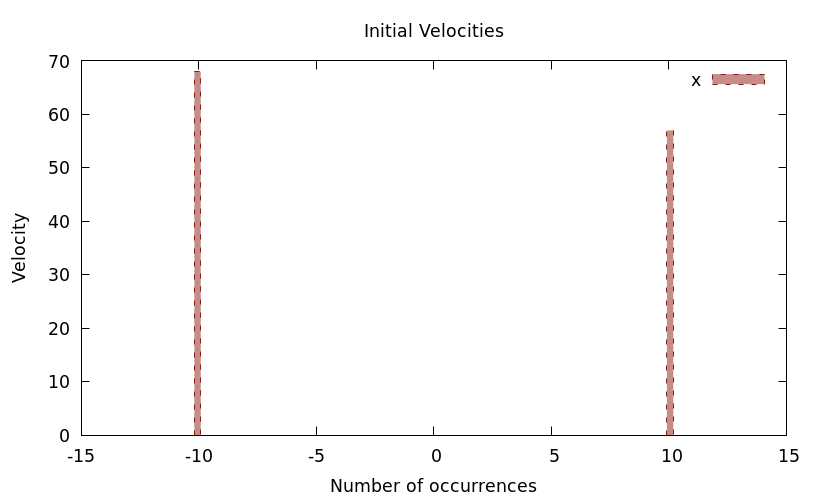
\includegraphics[width=\linewidth]{ini_vel_x}
		\caption{Eix x}
		\label{fig:ini_vel_x}
	\end{subfigure}
	\begin{subfigure}{0.3\linewidth}
		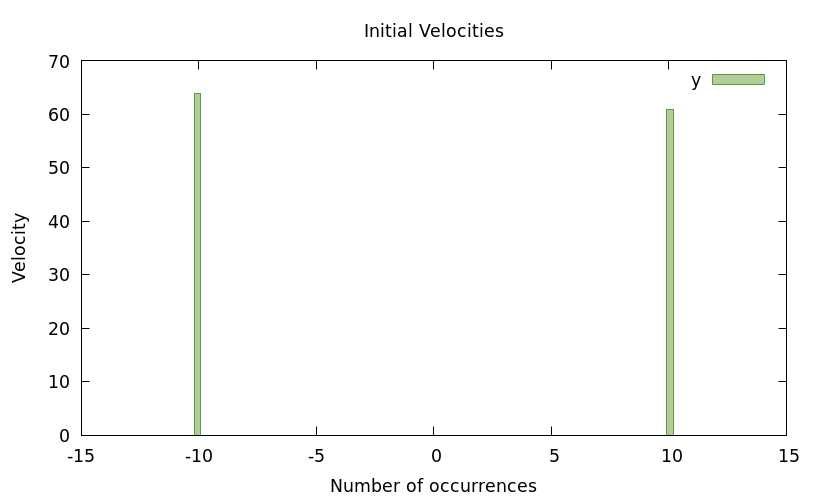
\includegraphics[width=\linewidth]{ini_vel_y}
		\caption{Eix y}
		\label{fig:ini_vel_y}
	\end{subfigure}
	\begin{subfigure}{0.3\linewidth}
		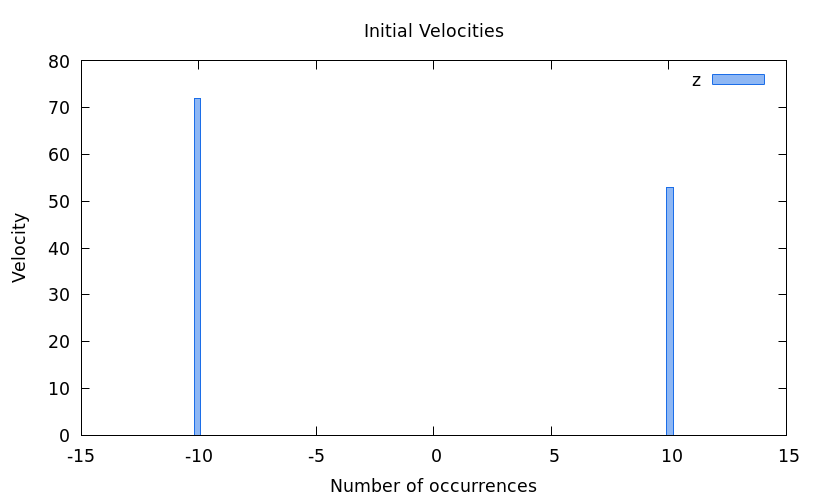
\includegraphics[width=\linewidth]{ini_vel_z} 
		\caption{Eix z}
		\label{fig:ini_vel_z}
	\end{subfigure}
	\caption{Distribució inicial de velocitats, per components.}
	\label{fig:ini_vel}
\end{figure}

Un cop equilibrat el sistema la distribució de velocitats hauria de ser similar a una distribució de Maxwell-Boltzmann. Tot i que aquest resultat prové de la teoria cinètica dels gasos i per tant s'aplica a gasos ideals clàssics, també es pot aplicar a gasos reals en temperatures ordinàries amb bons resultats \cite{StadPhys}. 

La distribució de Maxwell-Boltzmann és la següent:

\begin{equation}
	f(v) = \left[\frac{m}{2\pi k_b T}\right]^{3/2} 4\pi v^2 \exp\left(-\frac{mv^2}{2k_B T} \right)
\end{equation}

I per components:

\begin{equation}
	f(v_i) dv_i = \left[\frac{m}{2\pi k_b T}\right]^{1/2}  \exp\left(-\frac{mv_i^2}{2k_B T} \right) dv_i
\end{equation}

Veiem a la figura \ref{fig:fin_vel_verlet} com els nostres resultats concorden prou bé amb la teoria. L'histograma s'ha fet realitzant un promig dels 1000 darreres passos de temps. El sistema doncs s'ha desendreçat i ja no tenim una cúbica simple sinó un sistema gasós.

\begin{figure}
	\centering
	\begin{subfigure}{0.45\linewidth}
		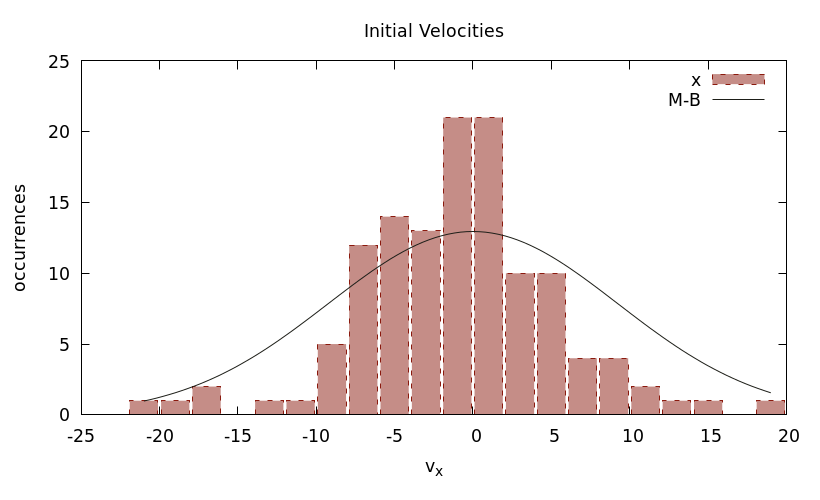
\includegraphics[width=\linewidth]{fin_vel_x_verlet}
		\caption{Eix x}
		\label{fig:fin_vel_x_verlet}
	\end{subfigure}
	\begin{subfigure}{0.45\linewidth}
		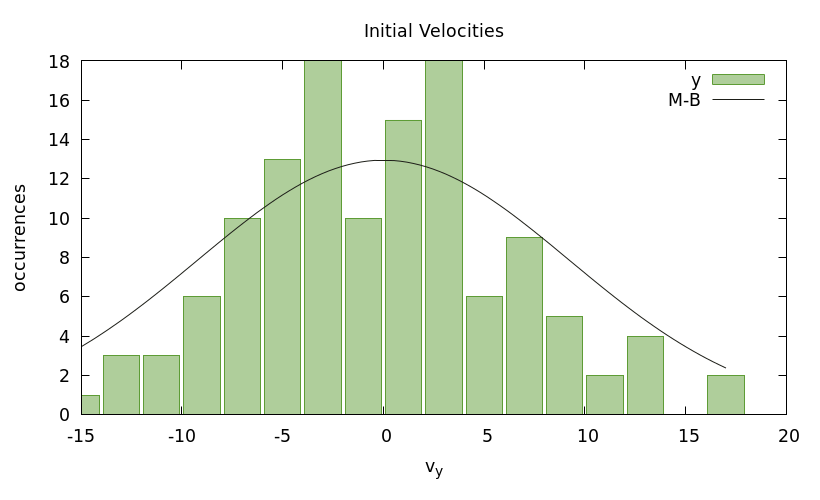
\includegraphics[width=\linewidth]{fin_vel_y_verlet}
		\caption{Eix y}
		\label{fig:fin_vel_y_verlet}
	\end{subfigure}
	\begin{subfigure}{0.45\linewidth}
		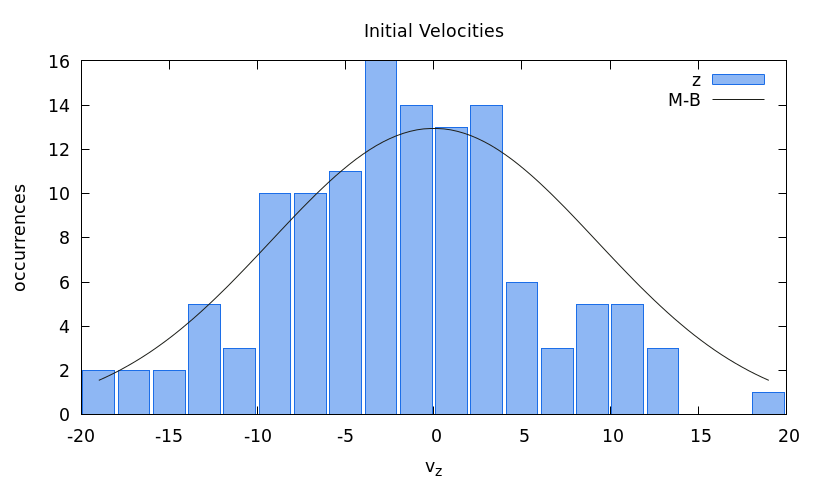
\includegraphics[width=\linewidth]{fin_vel_z_verlet} 
		\caption{Eix z}
		\label{fig:fin_vel_z_verlet}
	\end{subfigure}
	\begin{subfigure}{0.45\linewidth}	
		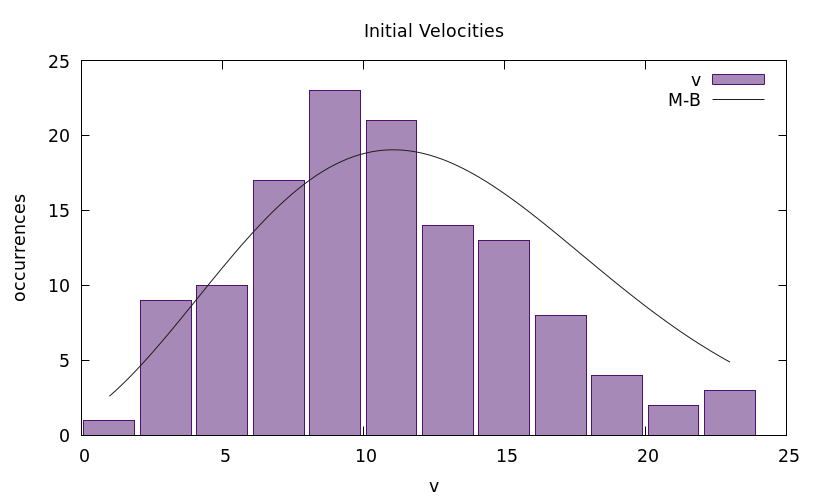
\includegraphics[width=\linewidth]{fin_vel_module_verlet} 
		\caption{Mòdul de la velocitat}
		\label{fig:fin_vel_module_verlet}
	\end{subfigure}
	\caption{Distribució final de velocitats, per components, ajustant una corba proporcional a la distribució de Maxwell-Boltzmann. Veiem que les nostres velocitats segueixen prou bé la distribució.}
	\label{fig:fin_vel_verlet}
\end{figure}

\section{Anàlisi de les propietats d'un líquid de Lennard-Jones}
En aquesta secció s'estudia la interacció entre àtoms d'Argó. Aquests tenen $\epsilon = 0.998$ kJ/mol i $\sigma = 3.4 \si{\angstrom}$.


% Calculate the kinetic, potential and total energy per particle of a system of (N > 100) argon atoms in a fluid state with densities ρ = 0.05, 0.1, 0.2, 0.4, 0.6, 0.8m/σ 3 and a fixed temperature (using a thermal bath) kB T = 1.2.

% • Plot a graph with the kinetic, potential and total energy as a function of density. Show your results in units of kJ/mol for the energies and g/cm3 for the density. How do you equilibrate your system? How many timesteps do you use to calculate your results?



\begin{figure}
	\centering
	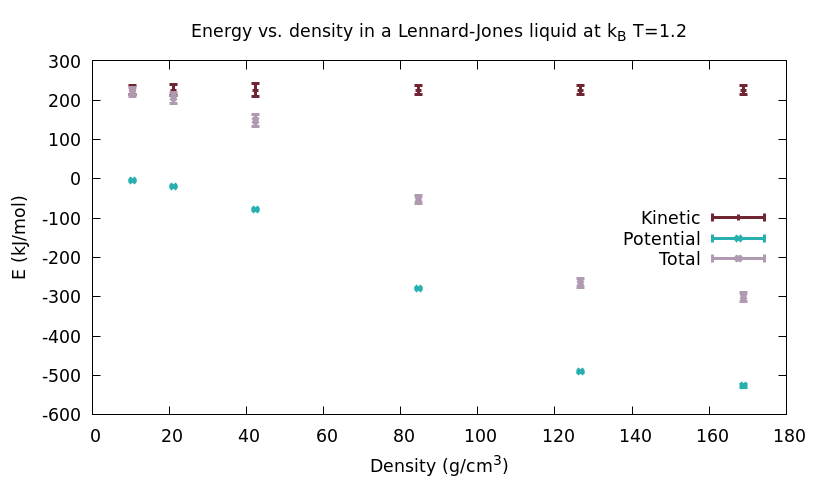
\includegraphics[width=\linewidth]{pot_energy_density}
	\caption{Promig de l'energia ciètica, potencial i total per diferents valors de la densitat, a temperatura fixa.}
	\label{fig:energyvsrho}
\end{figure}

Per fer-ho, s'ha inicialitzat el sistema de la mateixa manera que abans, amb una cúbica simple. Per desendreçar (fondre) el sistema, s'ha acoblat el sistema a un termòstat Andersen a $T' = 100$, i s'han dut a terme 10000 passos amb $\Delta t = 10^{-4}$ . A continuació s'ha rebaixat la temperatura a $T=1.2$ i s'han dut a terme 150.000 passos de producció. Aquest procés s'ha dut a terme pels següents valors de la densitat: $\rho' = 0.05, 0.1, 0.2, 0.4, 0.6, 0.8 $.


Tot fent ús del mètode de Block Average, s'han calculat l'energia cinètica, la potencial i la total del sistema. Els resultats obtingut es troben a la figura \ref{fig:energyvsrho}. En aquesta s'observa com l'energia cinètica del sistema es manté constant, ja que sempre estem treballant a la mateixa temperatura. Sabem, de física estadística, que la temperatura és un indicador de la velocitat de les partícules en un sistema. Per tant, com que l'energia cinètica té una estreta relació amb la velocitat, aquesta es manté constant en augmentar la densitat, ja que la temperatura del sistema no varia. D'altra banda, veiem com l'energia potencial minva amb la temperatura. Ens trobem en un sistema lligat, ja que l'energia potencial és negativa, i veiem com amb la densitat va augmentant el valor absolut de l'energia potencial. En augmentar la densitat les partícules seran més properes les unes amb les altres i per tant, l'energia potencial d'interacció serà major. 


També s'han calculat la pressió i la temperatura del sistema. Pel càlcul de la pressió s'ha seguit el capítol \textit{Simple termodinamical averages} de \cite{allen}. En aquest es defineix la pressió instantània com:

$$ \mathcal{P} = \rho k_b \mathcal{T} + \frac{\mathcal{W}}{V} \qquad \mathcal{W} = \frac{1}{3} \sum_i \sum_{j<i} r_{ij} f_{ij} $$ 

Aquesta quantitat s'ha acumulat i s'ha calculat fent-ne un promig amb el mètode de Block Average, com tota la resta de quantitats termodinàmiques. Encara que es van fer esforços per aconseguir resultats que es consideressin consistents, per certs valors de la densitat hem obtingut valors negatius de la pressió. S'ha comprovat la bibliografia (\cite{Hess}, \cite{Gregory}, \cite{HansenVerlet}) i s'ha vist que els nostres resultats concorden amb els seus i que per tant, tot i que el raonament físic escapa el nostre coneixement, sembla ser que els nostres resultats són acceptables. Cal mencionar que $T'=1.2$, com es pot veure a la figura \ref{fig:screenshot-from-2023-12-17-11-22-54}, per algunes densitats ens trobem a la zona de transició entre la fase gas i la fase líquida. Hi ha doncs una regió de coexistència de les dues fases, ja que és una transició de fase de segon ordre. Els valors estudiants pels quals s'obté una pressió menor que zero són en aquesta regió de coexistència. Així doncs, estem davant d'una transició de fase de gas a líquid. 


\begin{figure}
	\centering
	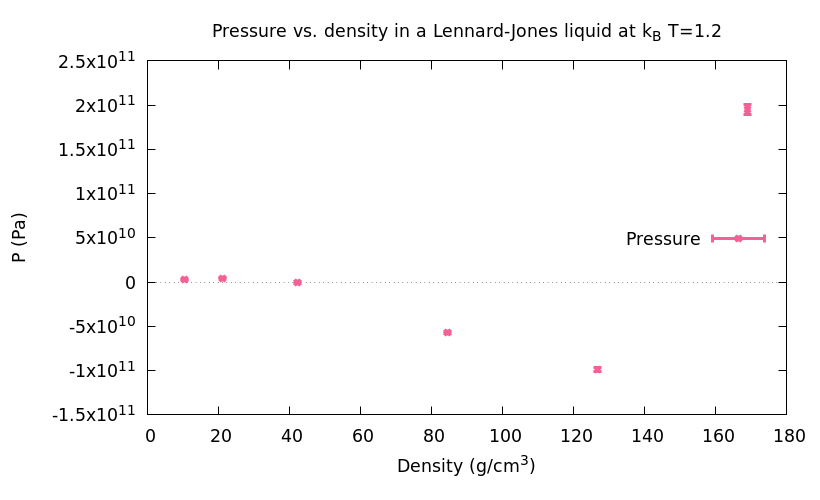
\includegraphics[width=1\linewidth]{preassure}
	\caption{Valors obtinguts de la pressió a diverses densitats.}
	\label{fig:preassure}
\end{figure}


	\begin{figure}
	\centering
	\includegraphics[width=\linewidth]{"../../../../../Pictures/Screenshots/Screenshot from 2023-12-17 11-11-40"}
	\caption{Font: \cite{Gregory}}
	\label{fig:screenshot-from-2023-12-17-11-11-40}
	\end{figure}

	\begin{figure}
		\centering
		\includegraphics[width=\linewidth]{"../../../../../Pictures/Screenshots/Screenshot from 2023-12-17 11-22-54"}
		\caption{Diagrama de fases d'un fluïd de Lennard-Jones. La zona vermella és la isoterma que estem explorant.}
		\label{fig:screenshot-from-2023-12-17-11-22-54}
	\end{figure}






% • Visualize (part of) the equilibrium trajectory and interpret your observations in terms of the phase diagram of the Lennard-Jones fluid shown in Fig. 1.



% Calculate the pressure of a system of (N > 100) argon atoms at kB T = 1.2 for densities ρ = 0.05, 0.1, 0.2, 0.4, 0.6, 0.8m/σ 3 . Plot your results in Pascal.

\section{Desplaçament quadràtic mitjà}

El desplaçament quadràtic mitjà (en anglès \textit{mean squared displacement}, MSD) és una mesura de la desviació de la posició de les partícules respecte una posició de referència. Representa una mesura quina part de l'espai ha estat recorreguda per una partícula: si una partícula es mou molt, el seu MSD serà elevat. En canvi, si una partícula està quieta, el seu MSD serà nul. Per calcular-lo, s'ha guardat la posició en la que es troba el sistema en acabar la inicialització, i a cada pas de temps s'ha calculat el MSD. Com amb la resta de mesures, s'ha fet servir la tècnica del Block Average. El resultat es mostra a la figura \ref{fig:msd}, on veiem que com era d'esperar, el MSD minva amb la densitat. A densitats baixes, les partícules tenen la capacitat de moure's molt, ja que estan menys lligades. Correspon a un comportament gasós. En canvi, quan la densitat augmenta i el sistema està en estat líquid, el desplaçament quadràtic mitjà és molt menor, ja que les partícules estan molt més lligades entre si, i tenen menys llibertat de moviment.


\begin{figure}
	\centering
	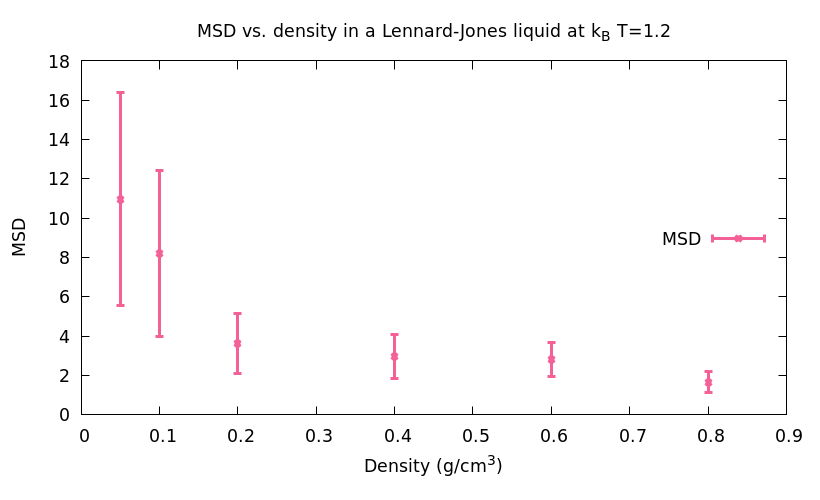
\includegraphics[width=\linewidth]{MSD}
	\caption{Desplaçament quadràtic mig en front de la densitat del sistema. }
	\label{fig:msd}
\end{figure}


\begin{figure}
	\centering
	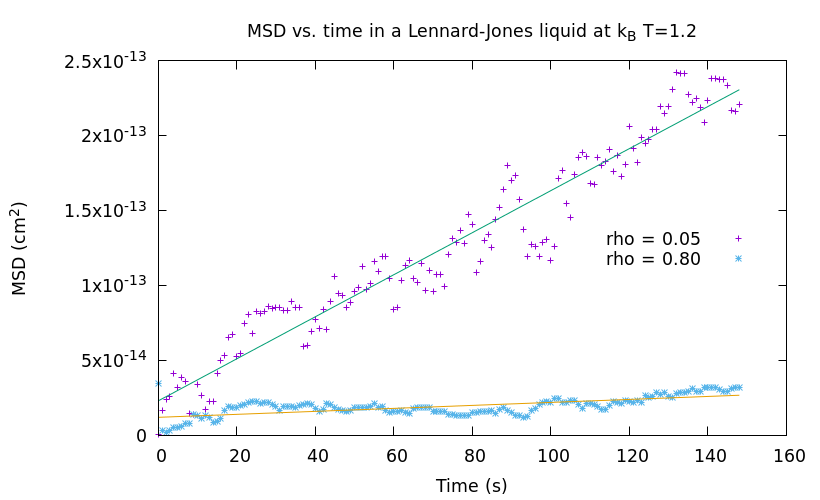
\includegraphics[width=\linewidth]{MSD_evol}
	\caption{Evolució del MSD en funció del temps per la fase gasosa ($\rho' = 0.05$) i la fase líquida ($\rho' = 0.80$).}
	\label{fig:msdevol}
\end{figure}

A la figura \ref{fig:msdevol} es veu l'evolució del MSD en funció del temps. S'ha fet un ajust lineal per obtenir el coeficient de difusió, ja que està relacionat amb el coeficient de difusió:

$$ \langle \Delta r(t)^2 \rangle \propto 6Dt $$ 

\begin{table}
	\centering
	\begin{tabular}{|c|c|c|}
		\hline
		$\rho'$ & $6D$ (cm$^2$/s) & $D$ (cm$^2$/s) \\
		\hline
		0.05 &  $(1.40 \pm 0.03) \times 10^{-15}$ & $(2.34 \pm 0.05 )\times 10^{-16}$ \\
		\hline
		0.80 &  $(10.0 \pm 0.9) \times 10^{-17}$ & $(1.66 \pm 0.12) \times 10^{-17}$\\
		\hline
	\end{tabular}
	\caption{Coeficients de difusió obtinguts per ambdues fases.}
	\label{tab:coeficients}
\end{table}

S'ha fet un ajust lineal de les dades i es relaciona el pendent amb 6t. Els resultats es troben a la taula \ref{tab:coeficients}. A la fase líquida ($\rho = 0.8$) el coeficient de difusió és un ordre de magnitud menor que en el gasós. 








\section{Conclusions}

\section{Annex}

\subsection{Inicialització de les posicions de les partícules}
\label{annex:inicialitzacio}
\begin{lstlisting}

Subroutine initialize_positions(N, rho, r)
! """"
! Calculates the positions r of N particles in a SC structure
! INPUTS: N, rho
! OUTPUT: r(N, 3)
! """"
	Implicit none
	integer, intent(in) :: N
	real(8), intent(in) :: rho
	real(8), dimension(N, 3), intent(out) :: r
	real(8) :: L, a, x, y, z, ini
	integer :: M, i, j, k, particle

	L = (N/rho)**(1./3.)

	M = N**(1./3.)

	a = L/(M)

	! Set the position of every particle
	particle = 1
	ini = -L/2.d0
	
	do i = 0, M-1
		do j = 0, M-1
			do k = 0, M-1
				x = ini + i*a
				y = ini + j*a
				z = ini + k*a
				r(particle, :) = (/x, y, z/)
				particle = particle + 1
			end do
		end do
	end do
End Subroutine
\end{lstlisting}

\subsection{Condicions periòdiques de contorn}
\label{annex:pbc}
\begin{lstlisting}

Subroutine pbc(vector, L, D)
	Implicit none
	integer :: D, i
	real(8), dimension(D), intent(inout) :: vector
	real(8), intent(in) :: L


	do i = 1, D
		if (vector(i).gt.L/2.) then
			vector(i) = vector(i) - L
			if (abs(vector(i)).gt.1000) then
				print*, "YOU HAVE INESTABILITIES!"
				stop 
			end if
		else if (vector(i).lt.(-L/2.)) then
			vector(i) = vector(i) + L
			if (abs(vector(i)).gt.1000) then
				print*, "YOU HAVE INESTABILITIES!"
				stop
			end if
		end if
	end do

Return
End Subroutine	
\end{lstlisting}

\subsection{Força emprant el potencial de Lennard-Jones}

\begin{lstlisting}
	
	Subroutine find_force_LJ(r, N, L, cutoff, F, pot)
		! """"
		! Calculates the forces applied to each particle of the system
		! INPUTS: r, Nm L, cutoff, F
		! OUTPUT: pot, F
		! """"
		Implicit none
		real(8), dimension(N, 3), intent(in) :: r
		real(8), intent(in) :: L, cutoff
		real(8) :: d, f_ij
		real(8), dimension(3) :: d_r
		integer :: i, j, k
		integer, intent(in) :: N
		real(8), dimension(N, 3), intent(out) :: F
		real(8), intent(out) :: pot
		
		pot = 0.d0
		
		F = 0.d0
		
		do i = 1, N
			do j = i+1, N
				d_r(:) = r(i, :) - r(j, :)
				
				do while (any(d_r(:).gt.L/2.).or.(any(d_r(:).lt.(-L/2.))))
					call pbc(d_r, L, size(d_r))
				end do
				
				
				d = (d_r(1)**2+d_r(2)**2+d_r(3)**2)**(1.d0/2.d0)
				if (d.le.cutoff) then
					f_ij = 48.d0 / d**14 - 24.d0 / d**8
					F(i,:) = F(i,:) + f_ij*d_r(:)
					F(j,:) = F(j,:) - f_ij*d_r(:)
				
				
						if (isnan(F(i,1))) then
							print*, i, j
							stop
						end if
				
					pot = pot + 4.d0*( 1.d0/ d**12 - 1.d0 /d**6) - 4.d0*( 1/ cutoff**12 - 1.d0 /cutoff**6)
				
				end if 
			
			end do
		end do
	
	End Subroutine
\end{lstlisting}

\subsection{Pas de temps de Velocity Verlet}
\begin{lstlisting}
	Subroutine time_step_vVerlet(r, vel, pot, N, L, cutoff, dt)
		! """"
		! Calculates a timestep using the velicity verlet algorithm
		! INPUTS: r, vel, N, L, cutoff, dt
		! OUTPUT: r, vel, pot
		! """"
		Implicit none
		integer, intent(in) :: N
		real(8), dimension(N, 3), intent(inout) :: r, vel
		real(8), intent(in) :: dt, L, cutoff
		real(8), dimension(N, 3) :: F
		real(8), intent(out) ::  pot
		integer :: i
	
		Call find_force_LJ(r, N, L, cutoff, F, pot)
	
		do i = 1, N
			r(i, :) = r(i, :) + vel(i, :) * dt + 0.5*F(i, :)*dt*dt
	
			do while (any(r(i,:) > L/2.) .or. any(r(i,:) < -L/2.))
			! Apply periodic boundary conditions using the pbc subroutine
				call pbc(r(i,:), L, size(r(i,:)))
			end do
	
	
			vel(i, :) = vel(i, :) + F(i, :)* 0.5 * dt
		end do
	
		Call find_force_LJ(r, N, L, cutoff, F, pot)
	
		do i = 1, N
			vel(i, :) = vel(i, :) + F(i, :)* 0.5 * dt
		end do
	
	
	End Subroutine
\end{lstlisting}

\subsection{Energia cinètica}

\begin{lstlisting}
	
	Subroutine kinetic_energy(vel, K_energy, N)
		Implicit none
		integer, intent(in) :: N
		real(8), dimension(N, 3) :: vel
		integer :: i, k
		real(8) :: K_energy
		
		K_energy = 0
		! for each particle
		do i = 1, N
			! loop over coordinates
			do k = 1, 3
				K_energy = K_energy + 0.5*vel(i,k)*vel(i,k) 
			end do
		end do
	End Subroutine
\end{lstlisting}

\subsection{Temperatura instantànea}
	\begin{lstlisting}
	Function inst_temp(N, K_energy)
		Implicit none
		integer :: N, N_f
		real(8) :: K_energy, inst_temp
		
		N_f = 3*N - 3
		inst_temp = 2.d0/(N_f)*K_energy
		Return
	End Function
	\end{lstlisting}	
	

\subsection{Inicialització de les velocitats}

\begin{lstlisting}

	Subroutine initialize_velocities(N, absV, vel)
	Implicit none
	integer, intent(in) :: N
	real(8) :: absV, rnd
	integer :: i, j
	real(8), dimension(N, 3) :: vel
	
	do i=1,N
		do j = 1,3
			call random_number(rnd)
			if (rnd.ge.0.5) then
				vel(i, j) = +absV
				else if (rnd.lt.0.5) then
				vel(i, j) = -absV
			end if
		end do
	end do
	
	
	End Subroutine
	
\end{lstlisting}

\subsection{Càlcul del moment total del sistema}

\begin{lstlisting}

	Subroutine momentum(vel, p, N)
		Implicit none
		real(8), dimension(N, 3) :: vel
		real(8), dimension(3) :: total_p
		integer :: N, i
		real(8), intent(out) :: p 
		
		total_p(:) = 0
		
		! Accumulate p
		do i = 1,N
		total_p(:) = total_p(:) + vel(i, :)
		end do
		
		! Produce the module
		p = ( total_p(1)**2 + total_p(2)**2 + total_p(3)**2 )**(1./2.) 
	
	
	End Subroutine
\end{lstlisting}



\subsection{Pas de temps Euler}
\begin{lstlisting}
	Subroutine time_step_Euler_pbc(r_in, r_out, vel, N, L, cutoff, dt, pot)
		Implicit none
		integer, intent(in) :: N
		real(8), dimension(N, 3), intent(in) :: r_in
		real(8), dimension(N, 3), intent(out) :: r_out
		real(8), dimension(N, 3) :: vel, F
		real(8), intent(in) :: L, dt
		integer :: i, counter
		real(8) :: cutoff, pot
		
		Call find_force_LJ(r_in, N, L, cutoff, F, pot)
		
		
		do i = 1, N
			r_out(i, :) = r_in(i, :) + vel(i, :) * dt + 0.5*F(i, :)*dt*dt
			vel(i, :) = vel(i, :) + F(i, :) * dt
			
			do while (any(r_out(i,:).gt.L/2.).or.(any(r_out(i,:).lt.(-L/2.))))
				call pbc(r_out, L, size(r_out))
			end do
			
		
		end do
	
	End Subroutine
\end{lstlisting}

\subsection{Pressió instantània}

\begin{lstlisting}
	Function W(N, r, rho, T, L, cutoff)
		Implicit none
		integer :: N, i, j, step
		real(8) :: suma, W, T, L, rho, d, cutoff, f_ij
		real(8), dimension(N,3) :: r
		real(8), dimension(3) :: r_ij
		
		suma = 0
		
		do i = 1, N
			do j = i+1, N
				r_ij(:) = r(i, :) - r(j, :)
				
				do while (any(r_ij(:).gt.L/2.).or.(any(r_ij(:).lt.(-L/2.))))
					call pbc(r_ij, L, size(r_ij))
				end do
				
				d = (r_ij(1)**2+r_ij(2)**2+r_ij(3)**2)**(1.d0/2.d0)
				
				if (d.le.cutoff) then
					f_ij = 48.d0 / d**13 - 24.d0 / d**7
					!	print*, "f", f_ij
					suma = suma + f_ij*d
				end if 
			
			end do
		end do
		
		! average = sum / (N*N)
		
		W = (1./3.)*suma
		
	
	end Function
	
\end{lstlisting}

\subsection{Desplaçament quadràtic mitjà}

\begin{lstlisting}
	Subroutine mean_sq_distance(r, r_0, N, MSD)
		Implicit none
		integer, intent(in) :: N
		real(8), dimension(N, 3), intent(in) :: r, r_0
		real(8), intent(out) :: MSD
		real(8) :: r_module, r_0_module
		integer :: i
		
		MSD = 0.d0
		
		do i = 1, N
			r_module = (r(i,1)**2 + r(i,2)**2 + r(i,3)**2)**2
			r_0_module =  (r_0(i,1)**2 + r_0(i,2)**2 + r_0(i,3)**2)**2
			MSD = MSD + (r_module - r_0_module)
		end do
		
		MSD = MSD/N
	
	End Subroutine
\end{lstlisting}



\subsection{Termòstat Andersen}

\begin{lstlisting}
	Subroutine therm_Andersen(vel, nu, sigma_gaussian, N)
		Implicit none
		integer :: i, N
		real(8) :: rand, nu, sigma_gaussian
		real(8), dimension(N, 3) :: vel
		real(8), dimension(2) :: xnums
		
		do i = 1, N
			call random_number(rand) 
				if (rand.lt.nu) then
					call BM(2, xnums, sigma_gaussian)
					!print*, "xnums: ", xnums
					vel(i, 1) = xnums(1)
					vel(i, 2) = xnums(2)
					call BM(2, xnums, sigma_gaussian)
					vel(i, 3) = xnums(1)
				end if
		end do
		!	print*, vel
	End Subroutine
\end{lstlisting}


\subsection{Box-Müller}

\begin{lstlisting}
	Subroutine BM(ndat,xnums,sigma)
		Implicit none
		Integer ::  ndat, i
		real(8), dimension(ndat) :: xnums
		real(8) :: r, phi, x1, x2, sigma
		real(8), parameter :: pi = 4.d0*atan(1.d0)
		
		Do i = 1, ndat, 2
			r = sqrt(-2.d0*log(1.d0-rand()))
			phi = 2.d0*pi*rand()
			x1 = r*cos(phi)
			x2 = r*sin(phi)
			if (i.ne.ndat) then ! Ens assegurem que no haguem acabat la llista
				xnums(i) = x1*sigma
				xnums(i+1) = x2*sigma
			endif
		end do
	return
	end Subroutine
	
\end{lstlisting}


\subsection{Processing code: compute average}

\begin{lstlisting}
import numpy as np
import os

# Function to calculate average and standard deviation for each column
def calculate_stats(data):
	averages = np.mean(data, axis=0)
	std_devs = np.std(data, axis=0)
	return averages, std_devs

# Read data from the file
file_path = os.environ.get("FILE")  # Replace with the actual path to your file
with open(file_path, 'r') as file:
	lines = file.readlines()

# Parse data from the lines
data = []
for line in lines:
	values = [float(val) for val in line.split()]
	data.append(values)

# Convert data to a NumPy array for easy calculations
data = np.array(data)

# Calculate averages and standard deviations
averages, std_devs = calculate_stats(data)

# Print the results
print(averages[0], std_devs[0], averages[1], std_devs[1], averages[2], std_devs[2], averages[3], std_devs[3], averages[4], std_devs[4])

\end{lstlisting}

\begin{lstlisting}
	#!/bin/bash
	
	for file in thermodynamics_*.dat; do
		echo "Processing file: $file"
		export FILE="$file"

		python3 compute_average.py >> results.dat
	done
	
\end{lstlisting}	

\begin{thebibliography}{100}
	\bibitem{StadPhys} Statistical Physics (2nd Edition), F. Mandl, Manchester Physics, John Wiley and Sons, 2008, ISBN 9780471915331
	\bibitem{vverlet} Swope, William C.; H. C. Andersen; P. H. Berens; K. R. Wilson (1 January 1982). "A computer simulation method for the calculation of equilibrium constants for the formation of physical clusters of molecules: Application to small water clusters". The Journal of Chemical Physics. 76 (1): 648 (Appendix).
	\bibitem{allen} Computer simulations of liquids, M.P. Allen and D.J. Tildesley, (Oxford Science Publications, 2000) 
	\bibitem{Hess} Hess, Siegfried. (1999). Augmented van der Waals equation of state for the Lennard-Jones fluid. Physica A: Statistical Mechanics and its Applications. 267. 58–70. 10.1016/S0378-4371(98)00670-0. 
	\bibitem{Gregory}: V. Paul Gregory, John C. Schug (1994): NPT Monte Carlo calculation of
	isotherms for the Lennard-Jones fluid, Molecular Physics: An International Journal at the Interface
	Between Chemistry and Physics, 82:4, 677-688
	\bibitem{HansenVerlet}  Hansen, J., and VerletT, L., Phase Transitions of the Lennard-Jones System, 1969, Phys. Rev., 184, 151

\end{thebibliography}


\end{document}